\documentclass{standalone}
\usepackage{tikz}

\begin{document}
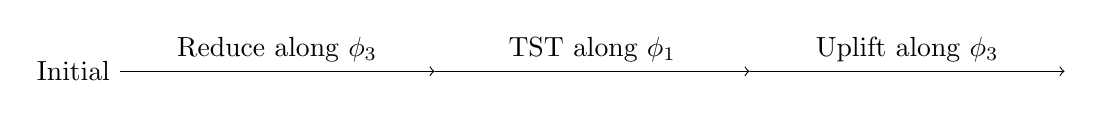
\begin{tikzpicture}[scale=2]
    % Define coordinates for nodes
    \coordinate (initial) at (0, 0);
    \coordinate (reduce_phi3) at (2, 0);
    \coordinate (TST_phi1) at (4, 0);
    \coordinate (uplift_phi3) at (6, 0);

    % Draw arrows between nodes with labels
    \draw[->] (initial) node[left] {Initial} -- (reduce_phi3) node[midway, above] {Reduce along $\phi_3$};
    \draw[->] (reduce_phi3) -- (TST_phi1) node[midway, above] {TST along $\phi_1$};
    \draw[->] (TST_phi1) -- (uplift_phi3) node[midway, above] {Uplift along $\phi_3$};

    % Add labels for clarity
    \node[below] at (initial) {};
    \node[below] at (reduce_phi3) {};
    \node[below] at (TST_phi1) {};
    \node[below] at (uplift_phi3) {};

\end{tikzpicture}
\end{document}